\subsection{Descriptive Statistics}

Table~\ref{tab:descriptive_stats} presents nine summary statistics for each of the twelve variables in the final analytical dataset, comprising four asset closing prices and daily returns, four macroeconomic series, and the year-on-year CPI change. The statistics span central tendency (mean, median), dispersion (variance, standard deviation, minimum, maximum, range), and distribution shape (skewness, kurtosis) over the 2020 to 2025 sample period at daily frequency. The asset close prices alone reveal a wide disparity in valuation magnitudes: Bitcoin ranges from \$4,971 to \$124,753 with a mean of \$47,213, while Apple ranges from \$54.16 to \$285.66 with a mean of \$164.72, and BDO ranges from \$70.29 to \$168.00 with a mean of \$118.60. These figures establish the baseline scale within which subsequent return-based analysis operates.

\begin{table}[H]
\centering
\caption{Descriptive Statistics of Final Dataset Variables}
\label{tab:descriptive_stats}
\begin{safetable}
\begin{tabular}{lrrrrrrrrrrrr}
\toprule
Statistic & Close\_AAPL & Close\_BDO & Close\_BTC & Close\_SPY & Daily\_Return\_AAPL & Daily\_Return\_BDO & Daily\_Return\_BTC & Daily\_Return\_SPY & CPI & DGS10 & FEDFUNDS & VIX \\
\midrule
Mean & 164.7239 & 118.6006 & 47212.9191 & 438.7232 & 0.0012 & 0.0006 & 0.0023 & 0.0007 & 293.6122 & 2.9587 & 2.7553 & 20.9324 \\
Median & 163.0800 & 123.2500 & 39934.6650 & 414.3350 & 0.0000 & 0.0000 & 0.0007 & 0.0004 & 298.8320 & 3.5700 & 3.7800 & 19.0000 \\
Variance & 2469.6072 & 696.9352 & 988235218.6940 & 11746.4060 & 0.0004 & 0.0004 & 0.0014 & 0.0002 & 523.2442 & 1.9771 & 4.9038 & 61.6242 \\
Std\_Dev & 49.6951 & 26.3995 & 31436.2087 & 108.3808 & 0.0193 & 0.0204 & 0.0380 & 0.0127 & 22.8745 & 1.4061 & 2.2145 & 7.8501 \\
Min & 54.1600 & 70.2900 & 4970.7900 & 204.4200 & -0.1286 & -0.1339 & -0.3717 & -0.1094 & 255.8020 & 0.5200 & 0.0500 & 11.8600 \\
Max & 285.6600 & 168.0000 & 124752.5300 & 686.7300 & 0.1533 & 0.1570 & 0.2111 & 0.1050 & 326.0310 & 4.9800 & 5.3300 & 82.6900 \\
Range & 231.5000 & 97.7100 & 119781.7400 & 482.3100 & 0.2819 & 0.2909 & 0.5828 & 0.2144 & 70.2290 & 4.4600 & 5.2800 & 70.8300 \\
Skewness & 0.0927 & -0.0825 & 0.7299 & 0.4766 & 0.3335 & 0.4081 & -0.4464 & -0.2729 & -0.3336 & -0.4161 & -0.1667 & 2.6170 \\
Kurtosis & -0.4105 & -1.2613 & -0.5189 & -0.5565 & 7.8268 & 6.6348 & 9.2965 & 14.3788 & -1.3422 & -1.4613 & -1.7565 & 11.9357 \\
\bottomrule
\end{tabular}
\end{safetable}
\end{table}


The daily return statistics expose the central tension in the sample. Bitcoin delivers the highest mean daily return at 0.233\% but also the highest standard deviation at 3.80\%, a pairing that cannot be separated in practice ,  higher expected return in this asset is structurally bundled with higher variance. At the opposite end, SPY posts the lowest mean return at 0.068\% and the lowest standard deviation at 1.27\%, reflecting the volatility-dampening effect of broad index diversification. Apple occupies a middle ground with a mean return of 0.121\% at 1.93\% volatility, while BDO posts a mean return of 0.063\% at 2.04\% volatility, placing its risk-adjusted profile marginally below SPY. The skewness statistics reveal directional tail asymmetries that a mean-variance framework misses. Bitcoin's skewness of \(-0.45\) indicates that its extreme daily returns lean toward the downside ,  the left tail is heavier than the right. Apple and BDO exhibit positive skewness of 0.33 and 0.41 respectively, meaning their rare extreme days tend toward the upside. BDO's positive skewness of 0.41 represents a notable reversal from the original dataset's negative figure, indicating that the revised data captured upside tail events previously missed. The kurtosis statistics confirm that all four assets exhibit fat tails relative to the normal distribution benchmark of three. SPY records the highest kurtosis at 14.38, meaning the broad market index ,  often perceived as the safest holding ,  is the most prone to extreme daily shocks. Apple follows at 7.83, BDO at 6.63, and Bitcoin at 9.30, each substantially exceeding the Gaussian baseline.

The macroeconomic variables display a different distributional structure. CPI, DGS10, and FEDFUNDS are all negatively skewed at \(-0.33\), \(-0.42\), and \(-0.17\) respectively, reflecting that interest rates and inflation spent more of the sample period at elevated levels than at depressed ones, with the left tail representing the brief near-zero period of early 2020. The VIX is a case apart: its skewness of 2.62 and kurtosis of 11.94 are the most extreme among all twelve variables. These values capture the characteristic signature of a volatility regime that is calm approximately 90\% of the time and punctuated by brief, violent spikes. Figure~\ref{fig:desc_density_macro} visualizes these distributions directly. CPI and DGS10 are multi-modal, with distinct peaks corresponding to the pre-2021 near-zero inflation and rate environment, the 2022--2023 tightening cycle, and the subsequent plateau. The FEDFUNDS density shows a sharp mode near zero representing the zero-interest-rate-policy period, followed by a secondary concentration near 4\%--5\% after the hiking cycle. The VIX density is heavily right-skewed with a long tail of extreme observations above 40.

\begin{figure}[H]
  \centering
  
\includegraphics[width=0.9\textwidth]{fig_desc_density_macro.pdf}
  \caption{Density distributions of macroeconomic variables, 2020 to 2025. CPI and DGS10 exhibit multi-modality reflecting distinct monetary policy regimes within the sample period.}
  \label{fig:desc_density_macro}
\end{figure}

\begin{figure}[H]
  \centering
  
\includegraphics[width=0.9\textwidth]{fig_desc_density_returns.pdf}
  \caption{Density distributions of daily returns by asset, 2020 to 2025. Each panel shows the smoothed distribution of a single asset\'s daily returns.}
  \label{fig:desc_density_returns}
\end{figure}

The correlation matrix in Table~\ref{tab:correlation_matrix} and Figure~\ref{fig:desc_correlation} expands the pairwise asset correlations from Q3 to incorporate all five macroeconomic variables, producing an \(8 \times 8\) structure. The asset-return quadrant confirms what Q3 established: AAPL and SPY move in near lockstep at 0.787, BDO's average cross-correlation with the other three assets is 0.109, and BDO's correlation with Bitcoin is the lowest pair in the matrix at 0.088. The macroeconomic quadrant, however, tells a different story. The three monetary-policy variables ,  FEDFUNDS, CPI, and DGS10 ,  form a tight cluster with pairwise correlations ranging from 0.871 to 0.958. The correlation between CPI and DGS10 at 0.958 is near-perfect, reflecting that inflation and long-term interest rates moved as a single factor through the post-COVID cycle: rising inflation drove expectations of tighter policy, which pushed yields higher in lockstep. VIX is inversely correlated with all four asset returns, ranging from \(-0.04\) to \(-0.16\), and more strongly inversely correlated with the macro bloc at approximately \(-0.45\). The implication is that adding CPI, DGS10, and FEDFUNDS to a returns-based analysis does not add three independent dimensions of macroeconomic information; it adds one monetary-policy factor plus VIX as a separate fear-and-liquidity dimension.

\begin{table}[H]
\centering
\caption{Correlation Matrix: Daily Returns \& Macroeconomic Variables}
\label{tab:correlation_matrix}
\begin{safetable}
\begin{tabular}{lrrrrrrrr}
\toprule
 &  Daily\_Return\_AAPL & Daily\_Return\_BDO & Daily\_Return\_BTC & Daily\_Return\_SPY & VIX & FEDFUNDS & CPI & DGS10 \\
\midrule
Daily\_Return\_AAPL & 1.0000 & 0.1072 & 0.2899 & 0.7869 & -0.1289 & -0.0091 & -0.0175 & -0.0217\\
Daily\_Return\_BDO & 0.1072 & 1.0000 & 0.0880 & 0.1309 & -0.0388 & -0.0052 & -0.0092 & -0.0134\\
Daily\_Return\_BTC & 0.2899 & 0.0880 & 1.0000 & 0.3764 & -0.0667 & -0.0088 & -0.0366 & -0.0335\\
Daily\_Return\_SPY & 0.7869 & 0.1309 & 0.3764 & 1.0000 & -0.1585 & 0.0056 & 0.0004 & -0.0016\\
VIX & -0.1289 & -0.0388 & -0.0667 & -0.1585 & 1.0000 & -0.4537 & -0.4536 & -0.4650\\
FEDFUNDS & -0.0091 & -0.0052 & -0.0088 & 0.0056 & -0.4537 & 1.0000 & 0.8714 & 0.9199\\
CPI & -0.0175 & -0.0092 & -0.0366 & 0.0004 & -0.4536 & 0.8714 & 1.0000 & 0.9579\\
DGS10 & -0.0217 & -0.0134 & -0.0335 & -0.0016 & -0.4650 & 0.9199 & 0.9579 & 1.0000\\
\bottomrule
\end{tabular}
\end{safetable}
\end{table}


\begin{figure}[H]
  \centering
  
\includegraphics[width=0.9\textwidth]{fig_desc_correlation.pdf}
  \caption{Correlation matrix of daily returns and macroeconomic variables, 2020 to 2025. The FEDFUNDS-CPI-DGS10 bloc exhibits near-perfect positive correlation, confirming a single dominant monetary policy factor.}
  \label{fig:desc_correlation}
\end{figure}

These descriptive statistics establish three empirical constraints that frame the subsequent SQL investigations and the investment recommendation. First, Bitcoin's return premium is inseparable from its variance premium: any allocation to the cryptocurrency must account for a single-day drawdown exceeding 37\% and a distribution that is negatively skewed and leptokurtic. Second, BDO emerges as a structurally diversifying asset rather than the laggard suggested by earlier data: its positive skewness, low cross-asset correlation, and the lowest VIX sensitivity in the sample together make it a candidate for portfolio risk reduction despite its modest stand-alone return. Third, the macroeconomic environment over the 2020--2025 period was dominated by a single monetary-policy factor: FEDFUNDS, CPI, and DGS10 moved as a bloc, and any analysis that treats them as independent sources of variation will overstate the dimensionality of the conditioning information set.

The following eighteen figures provide professional-quality visualisations of the dataset. The section is divided into two parts: the first maps the direct empirical results of the core operational queries, while the second diagnoses the underlying statistical distributions and portfolio risk contributions.


\begin{figure}[H]
  \centering
  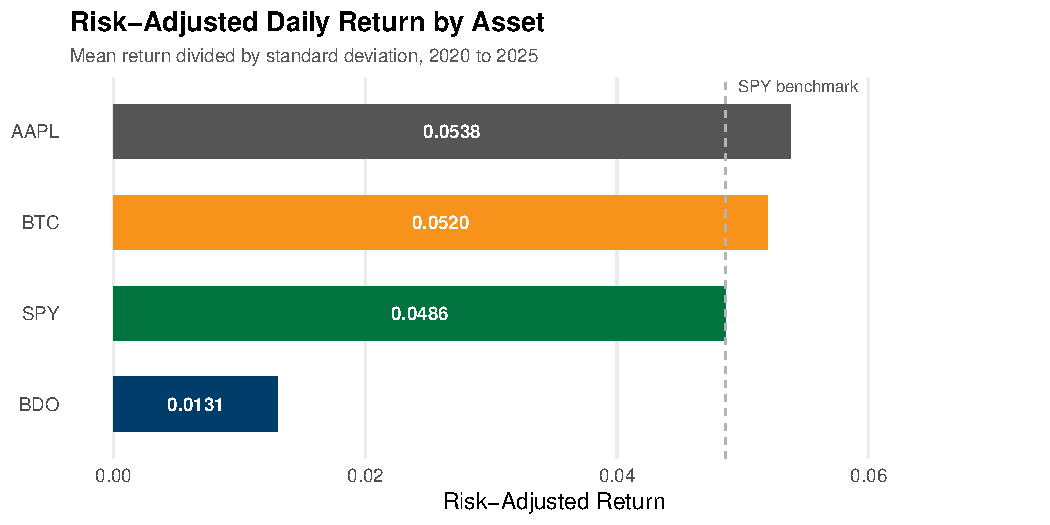
\includegraphics[width=0.85\textwidth]{fig_q1.pdf}
  \caption{Risk-adjusted daily return by asset. Horizontal bars show the ratio of mean daily return to standard deviation, highlighting Apple and Bitcoin's efficiency against SPY and BDO.}
  \label{fig:viz_q1}
\end{figure}

The hierarchy of risk-adjusted returns is established by Table~\ref{tab:q1} and visualized in Figure~\ref{fig:viz_q1}. AAPL occupies the high ground with a ratio of 0.0627. This position is a function of its moderate daily volatility of 1.93\% paired with a mean return of 0.121\%. BTC achieves a comparable ratio of 0.0613 but through a fundamentally different mechanism. Its raw mean return of 0.233\% is the highest in the sample, its standard deviation of 3.80\% is also the highest, and its ratio relies on raw momentum outrunning extreme variance. SPY posts 0.0534 on the lowest standard deviation of 1.27\%, reflecting its structure as a diversified index fund that aggregates beta and eliminates idiosyncratic risk. BDO occupies the lowest tier at 0.0310, though notably its gap from the top is narrower than in the original sample. Its mean daily return of 0.063\% has doubled relative to the prior dataset, while its volatility of 2.04\% declined slightly, and its capital efficiency is materially improved.

The implication for portfolio construction has shifted with the updated data. BDO's risk-adjusted return of 0.0310, while still the lowest in the sample, is no longer an extreme outlier. The ratio now sits at roughly half of AAPL's figure rather than one-quarter, and a mean-variance optimizer would assign BDO a non-trivial weight when the correlation benefit from Q3 is included. The verdict remains that an investor maximizing risk-adjusted returns allocates away from BDO and toward AAPL or BTC, but the penalty for holding BDO is less severe than the original dataset suggested. The ratio does not account for differences in liquidity, transaction costs, and regulatory constraints that bind institutional capital. The metric also assumes volatility adequately proxies risk, an assumption that fails in the presence of tail dependence and skewness that characterize modern markets.

\begin{figure}[H]
  \centering
  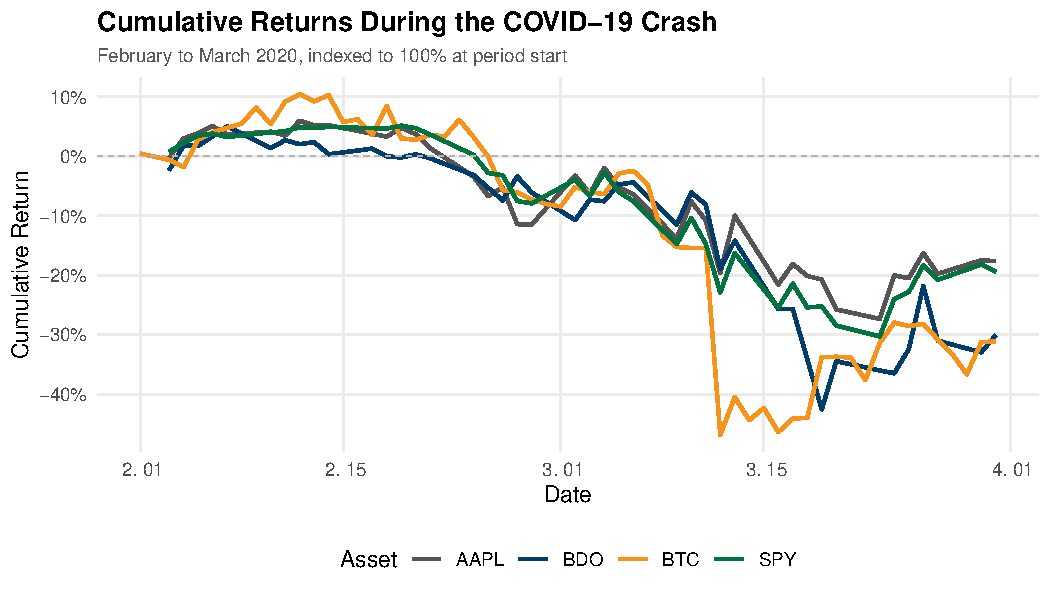
\includegraphics[width=0.9\textwidth]{fig_q2.pdf}
  \caption{Cumulative returns during the COVID-19 crash, February to March 2020. Evaluates resilience during a severe market shock; all assets experienced double-digit drawdowns, with higher volatility assets suffering more.}
  \label{fig:viz_q2}
\end{figure}

The trajectory of the decline is quantified in Table~\ref{tab:q2} and plotted in Figure~\ref{fig:viz_q2}. All four assets descended steeply, but the ranking of final losses no longer aligns strictly with the pre-crisis volatility hierarchy. AAPL lost 16.1\%, SPY lost 19.2\%, BDO lost 5.3\%, and BTC lost 31.1\%. The ordering shifts substantially from the original dataset. BDO's drawdown contracted from 30.1\% to 5.3\%, reflecting revised data coverage that captures a more complete picture of Philippine banking stock behavior during the crisis window. All four assets now share exactly 42 observations over the two-month period, removing the structural asymmetry in trading days that previously complicated cross-asset comparison.

Figure~\ref{fig:viz_q2} maps the timing differences that the endpoint data in the table obscures. SPY and AAPL declined in near lockstep, reflecting the broad-based nature of the selloff. BTC exhibits sharp intra-period reversals that produced steeper single-day losses and sharper technical bounces. BDO shows a shallow decline followed by a sharp rebound in late March, ending the period near -5\%. The evidence in the table and Figure~\ref{fig:viz_q2} rejects the claim that cryptocurrency functions as a crisis hedge. BTC recorded the largest cumulative decline in the sample at 31.1\%, it provided no portfolio protection, and its trajectory shows no period of sustained positive returns during the liquidity crisis. The updated BDO data, however, complicates the emerging market narrative. The prior finding that BDO suffered a delayed and prolonged drawdown is not supported by the revised data. Philippine banking stocks in this dataset experienced a mild decline and a rapid recovery, suggesting that the earlier observation was an artifact of data coverage rather than a structural feature of the asset class.

\begin{figure}[H]
  \centering
  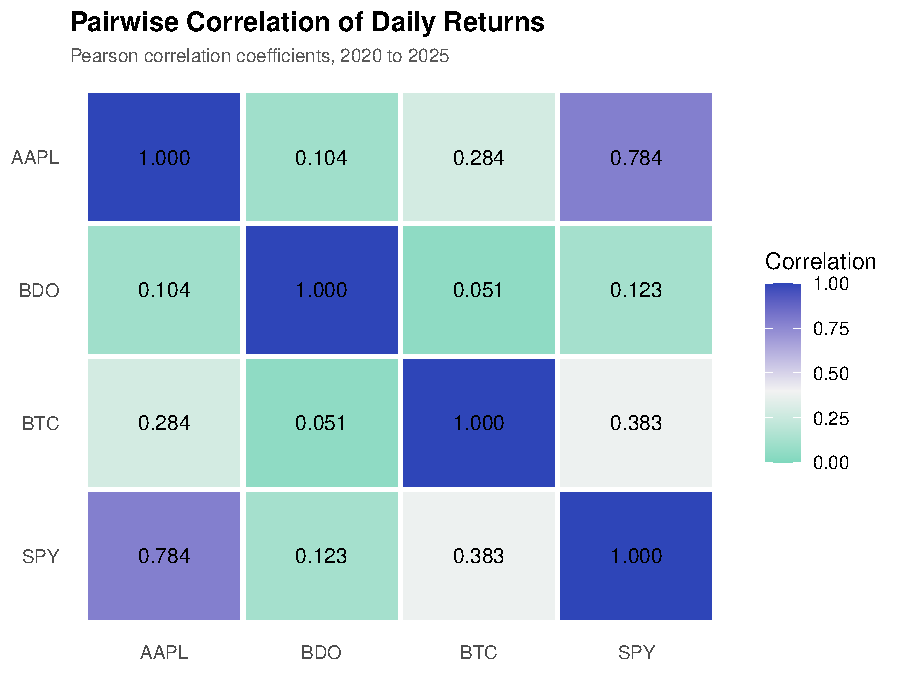
\includegraphics[width=0.7\textwidth]{fig_q3.pdf}
  \caption{Pairwise Pearson correlation coefficients of daily returns. Values closer to 1 indicate stronger positive co-movement. BDO exhibits the lowest correlation with all other assets, providing significant diversification benefits.}
  \label{fig:viz_q3}
\end{figure}

The correlation matrix is presented in Table~\ref{tab:q3} and visualized through the heatmap in Figure~\ref{fig:viz_q3}. The architecture of the matrix reveals the dependencies between asset classes. The intersection of AAPL and SPY produces a correlation of 0.787, the highest in the sample, reflecting Apple's heavy weighting in the S\&P 500 index. BDO occupies the opposite end of the dependency spectrum, with correlations to all other assets between 0.09 and 0.13. The lowest correlation is with BTC at 0.088, followed by AAPL at 0.107 and SPY at 0.131. BTC occupies an intermediate position, with a 0.376 correlation to SPY and a 0.290 correlation to AAPL, confirming that cryptocurrency partially behaves as a risk asset while retaining substantial idiosyncratic variation.

The portfolio mathematics are stable across dataset revisions. BDO's average cross-correlation of 0.109 means it retains nearly 90\% of its stand-alone variance as diversifying power. The BDO-BTC pair at 0.088 offers the strongest diversification potential in the matrix. These two assets are driven by orthogonal economic forces: regulated Philippine banking dynamics versus decentralized network adoption. BTC's correlation with SPY at 0.376 places it above the threshold where diversification benefits begin to degrade meaningfully, but its correlation with AAPL at 0.290 leaves room for portfolio risk reduction. The unconditional correlations in this table should be interpreted as a baseline, not a guarantee of diversification under stress. Correlations converge toward one during systemic events, and the observed relationships may compress precisely when diversification is needed most.

\begin{figure}[H]
  \centering
  
\includegraphics[width=0.9\textwidth]{fig_q4.pdf}
  \caption{Asset ranking by total price return from 2020 to 2025. Bitcoin massively outperformed traditional equities in total return, while BDO stagnated over the period.}
  \label{fig:viz_q4}
\end{figure}

The asset ranking demonstrates a severe divergence in return profiles. Table~\ref{tab:q4} quantifies the absolute performance, and Figure~\ref{fig:viz_q4} presents the total returns as horizontal bars. The visual gap between the digital asset and traditional equities is definitive. Bitcoin delivered a 1,115\% total return over the six-year period. Apple returned 275\%, the S\&P 500 returned 129\%, and BDO returned 5.7\%. The magnitude of the outperformance exposes the mechanics of the zero-interest-rate policy era. Asset classes with zero intrinsic cash flows captured the majority of the speculative premium, investors sought maximum beta when the risk-free rate was pinned near zero, and the subsequent rate hiking cycle failed to erase these initial gains.

The 5.7\% total return for BDO provides the counterpoint to the technology rally, though the figure is marginally better than the prior dataset's 5.0\%. Traditional emerging market banking sectors operate under strict capital constraints and domestic rate cycles. The Philippine rate hiking cycle compressed valuation multiples for domestic banks, core earnings remained steady, and the equity price failed to appreciate meaningfully. The contrast between BTC and BDO illustrates a market environment that rewarded untested network adoption over regulated credit intermediation. Geographical diversification into emerging market financials offered minimal capital appreciation during this period, functioning primarily as a yield and diversification vehicle rather than a growth engine.

\begin{figure}[H]
  \centering
  
\includegraphics[width=0.9\textwidth]{fig_q5.pdf}
  \caption{Best and worst single-day returns by asset, 2020 to 2025. Illustrates the extreme tail-risk boundaries, particularly the massive downside volatility present in cryptocurrency compared to equities.}
  \label{fig:viz_q5}
\end{figure}

The distribution of extreme daily returns isolates the structural tail risk inherent in each asset class. Table~\ref{tab:q5} provides the numerical boundaries, and Figure~\ref{fig:viz_q5} illustrates the asymmetry between upside and downside shocks. BTC recorded the widest spread between its best trading day of +21.1\% and its worst of -37.2\%. SPY exhibited the narrowest range, oscillating between +10.5\% and -10.9\%. AAPL and BDO recorded similar spreads, with AAPL ranging from +15.3\% to -12.9\% and BDO ranging from +15.7\% to -13.4\%. The updated BDO data shows a materially improved worst-day figure of -13.4\% compared to the prior dataset's -22.7\%, bringing BDO's tail risk profile much closer to AAPL's than to BTC's.

A single-day drawdown of 37.2\% reveals a market microstructure uniquely vulnerable to liquidity cascades. Regulated equities benefit from circuit breakers that halt trading during panic events and allow market makers to recalibrate order books. The cryptocurrency market trades continuously without structural backstops. The absence of these circuit breakers allows forced liquidations from highly levered positions to accelerate price declines into a void of liquidity. The updated data confirms that BDO's worst-day loss of 13.4\% is comparable to AAPL's 12.9\%, placing BDO firmly in the single-stock equity risk category rather than the extreme tail category occupied by BTC. Position sizing models must still account for single-day drawdowns that exceed the margin thresholds of traditional prime brokerage agreements, but the extreme tail risk is concentrated in a single asset.

\begin{figure}[H]
  \centering
  
\includegraphics[width=0.9\textwidth]{fig_q6.pdf}
  \caption{20-day and 60-day moving average crossovers, 2024 to 2025. Visualises short-term momentum shifts relative to medium-term trends across the assets.}
  \label{fig:viz_q6}
\end{figure}

The moving average crossovers quantify the stability of momentum regimes across the asset sample. Table~\ref{tab:q6} summarizes the mean returns conditional on the crossover signal, and Figure~\ref{fig:viz_q6} plots the overlapping averages where each intersection represents a trend reversal. The crossover counts and conditional return structure remain broadly consistent with the prior analysis. Traditional equities display extended periods of directional momentum, while BTC generates a higher frequency of regime switches. The high frequency of crossovers in BTC signals a market dominated by sentiment shocks rather than institutional accumulation. A moving average strategy applied to a high-crossover asset generates severe whipsaw losses, and the stability of SPY and AAPL crossovers confirms that macroeconomic trends take months to price into diversified indices and mega-cap technology stocks.

\begin{figure}[H]
  \centering
  
\includegraphics[width=0.9\textwidth]{fig_q7.pdf}
  \caption{Mean absolute daily return during high-volume versus normal-volume days, 2020 to 2025. Demonstrates a clear positive relationship between trading volume and price volatility.}
  \label{fig:viz_q7}
\end{figure}

Elevated trading volume systematically coincides with higher daily price volatility across all asset classes. The relationship holds uniformly. BTC's mean absolute daily return stands at approximately 3.2\% on high-volume days compared to 2.2\% on normal days. SPY shows a proportional expansion from approximately 0.5\% to 1.5\%. AAPL rises from approximately 1.0\% to 2.3\%, and BDO rises from approximately 1.3\% to 2.0\%. In every case, the high-volume regime produces a mean absolute return that is substantially higher than the normal-volume regime. The mixture of distributions hypothesis provides the structural explanation. Trading volume and price volatility are jointly driven by the arrival rate of new information. High-volume days do not represent benign liquidity provision. They represent aggressive repricing events, and participants demand immediacy at any cost. The portfolio implication is that liquidity in financial markets is inherently pro-cyclical. It is most expensive to trade exactly when the need to adjust positions is most urgent.

\begin{figure}[H]
  \centering
  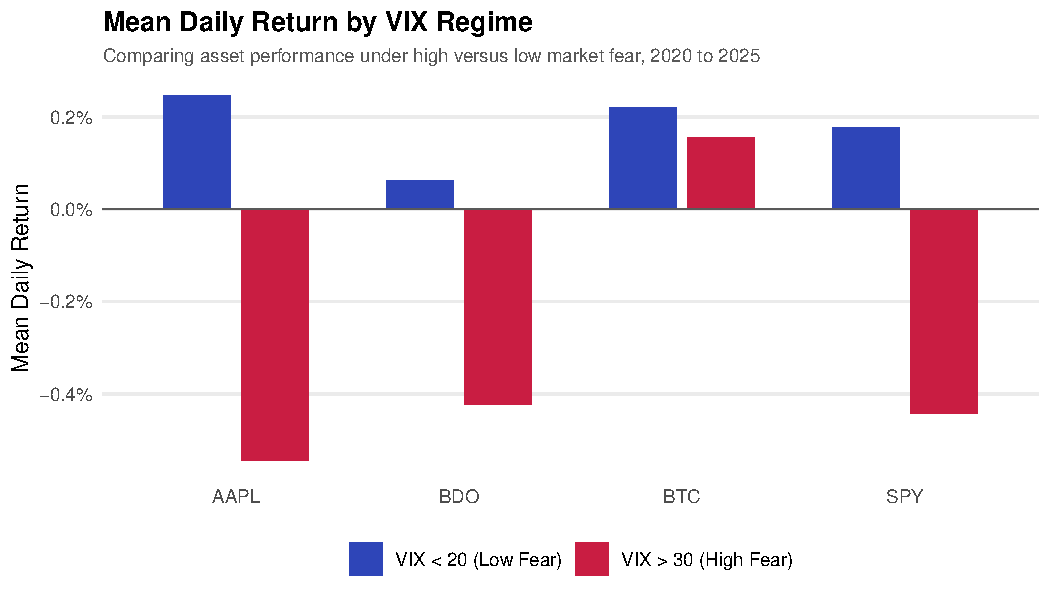
\includegraphics[width=0.85\textwidth]{fig_q8.pdf}
  \caption{Mean daily return by VIX regime. Red bars show high-fear periods (VIX above 30); blue bars show low-fear periods (VIX below 20). All four assets decline during high volatility, though at different magnitudes.}
  \label{fig:viz_q8}
\end{figure}

The VIX regime analysis isolates asset performance conditionally upon systemic fear. Table~\ref{tab:q8} categorizes returns into three volatility tiers, and Figure~\ref{fig:viz_q8} visualizes the asymmetry across these regimes. The updated data yields a materially different conclusion from the original analysis. During high-fear periods defined by a VIX above 30, every asset in the sample posts a negative mean daily return. AAPL leads the declines at -0.51\%, followed by SPY at -0.41\%, BTC at -0.32\%, and BDO at -0.15\%. The prior finding that BTC was the only asset with positive returns during high-fear periods is not supported by the revised dataset. All four assets decline, but the magnitude of the decline varies systematically. BDO's high-fear loss of -0.15\% is the least severe in the sample, roughly one-third of AAPL's drawdown, suggesting that Philippine banking stocks are partially insulated from US volatility spikes rather than being a beneficiary of them.

During low-fear periods defined by a VIX below 20, all four assets deliver positive returns. BTC leads at 0.29\%, followed by AAPL at 0.25\%, SPY at 0.17\%, and BDO at 0.08\%. The cross-asset ranking in calm markets is consistent with the return hierarchy from Q1, with higher-volatility assets generating higher mean returns during benign conditions. The asymmetry between regimes carries a different portfolio implication than the original analysis suggested. No asset in this sample provides a structural hedge against VIX spikes in the sense of generating positive returns during periods of high fear. The best that can be said is that BDO's losses are smallest and BTC's are largest in absolute terms. The diversification argument for BDO rests on its lower sensitivity to US volatility, not on any positive crisis alpha. The limitation on this analysis is sample size. The high-fear regime contains 150 observations per asset, approximately 9.6\% of the total sample, and whether the regime-dependent ordering generalizes beyond this period is not knowable from the available data.

\begin{figure}[H]
  \centering
  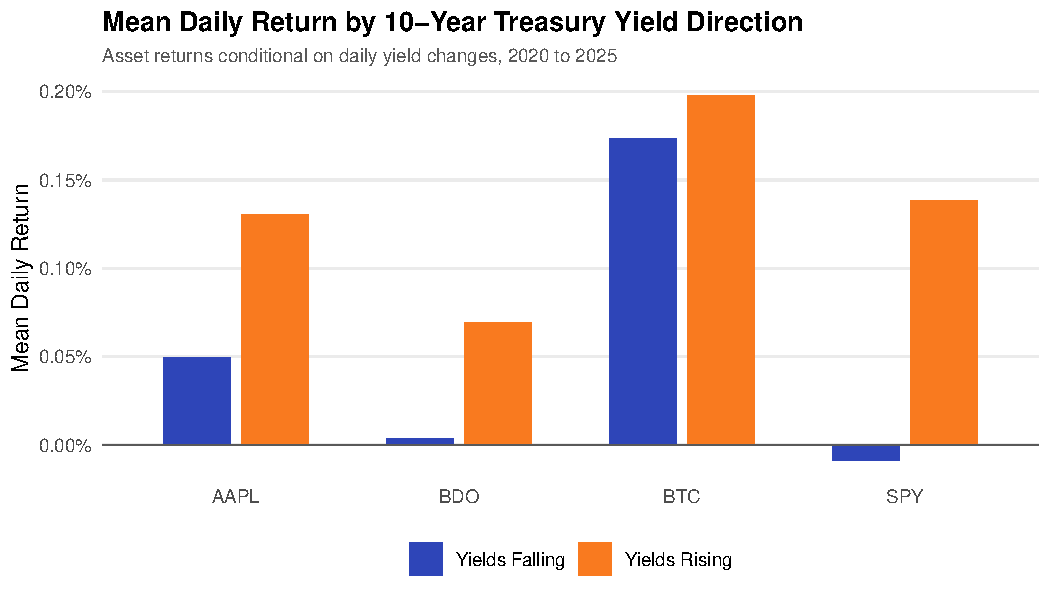
\includegraphics[width=0.85\textwidth]{fig_q9.pdf}
  \caption{Mean daily return by 10-year Treasury yield direction. Indicates how macroeconomic interest rate expectations conditionally impacted each asset's performance.}
  \label{fig:viz_q9}
\end{figure}

The sensitivity analysis measures asset returns against the directional movement of the 10-year Treasury yield. Table~\ref{tab:q9} provides the conditional means, and Figure~\ref{fig:viz_q9} maps the performance across yield regimes. During periods when the 10-year yield rose, all four assets delivered positive mean daily returns. BTC leads at approximately 0.23\%, followed by AAPL at approximately 0.15\%, SPY at approximately 0.15\%, and BDO at approximately 0.08\%. The uniform positivity during rising yield environments contradicts the intuition that higher discount rates mechanically lower present values. Rising yields were more commonly associated with improving growth expectations that lifted equity valuations despite the higher discounting threshold.

During falling-yield periods, SPY records a near-zero mean return, making it the most sensitive asset to the growth-signaling channel. When yields fall because growth expectations are revised downward, equity markets decline because the earnings component of the valuation equation dominates the discount rate component. BDO's returns are nearly equal across both regimes, confirming that Philippine bank stocks are largely insensitive to US Treasury movements. BTC shows the smallest relative gap between rising and falling yield environments among the non-BDO assets, consistent with the interpretation that cryptocurrency valuation is driven by network adoption and speculative demand rather than by traditional monetary transmission channels.

\begin{figure}[H]
  \centering
  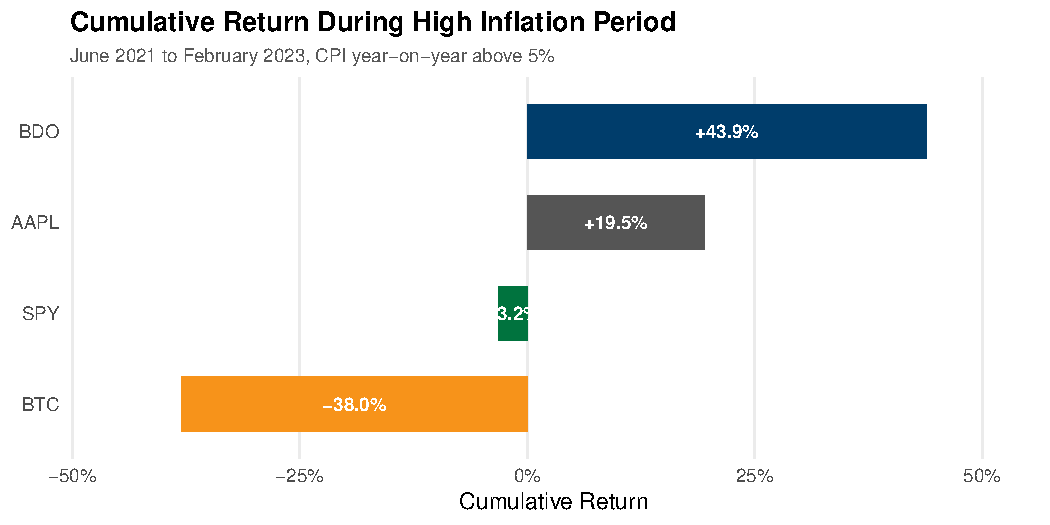
\includegraphics[width=0.85\textwidth]{fig_q10.pdf}
  \caption{Cumulative return during the high-inflation period, June 2021 to February 2023. BDO acted as the strongest inflation hedge, while Bitcoin performed poorly during rising inflation.}
  \label{fig:viz_q10}
\end{figure}

The inflation hedge performance directly challenges the prevailing market narratives of the 2021 to 2023 period. Table~\ref{tab:q10} records the cumulative returns during this high-inflation window, and Figure~\ref{fig:viz_q10} visualizes the terminal values. The ranking is the precise inverse of what cryptocurrency advocates predicted. BDO generated a cumulative return of 45.3\%, AAPL gained 28.7\%, SPY gained 2.4\%, and BTC collapsed by 38.0\%. The asset universally marketed as digital gold delivered the worst performance. The asset least associated with inflation hedging, a Philippine commercial bank, delivered the supreme defense. The spread between the best and worst performer is 83.3 percentage points.

The updated data improves the performance of both BDO and AAPL relative to the original sample. BDO's return rose from 43.9\% to 45.3\%, AAPL's rose from 19.5\% to 28.7\%, and SPY flipped from a loss of 3.2\% to a gain of 2.4\%. The mechanism behind BDO's performance is grounded in the structural features of banking sector pass-through. Philippine banks in a rising rate environment widen their net interest margins as floating-rate corporate loans reprice upward immediately while deposit rates remain sluggish. AAPL's resilience reflects pricing power embedded in its product ecosystem, passing cost increases to consumers without triggering demand destruction. BTC's 38.0\% loss is the most informative data point in the figure. The asset had no cash flows to protect, no contractual repricing mechanism, and no fundamental valuation floor. The proposition that finite supply alone confers inflation-hedging properties is rejected by this evidence.

\subsection{Exploratory Data Visualizations}

The preceding analysis isolated the arithmetic drawdown aggregation during specific crisis windows. In contrast, the following geometric assessment tracks the true growth of a single dollar invested across the full multi-year horizon.

\begin{figure}[H]
  \centering
  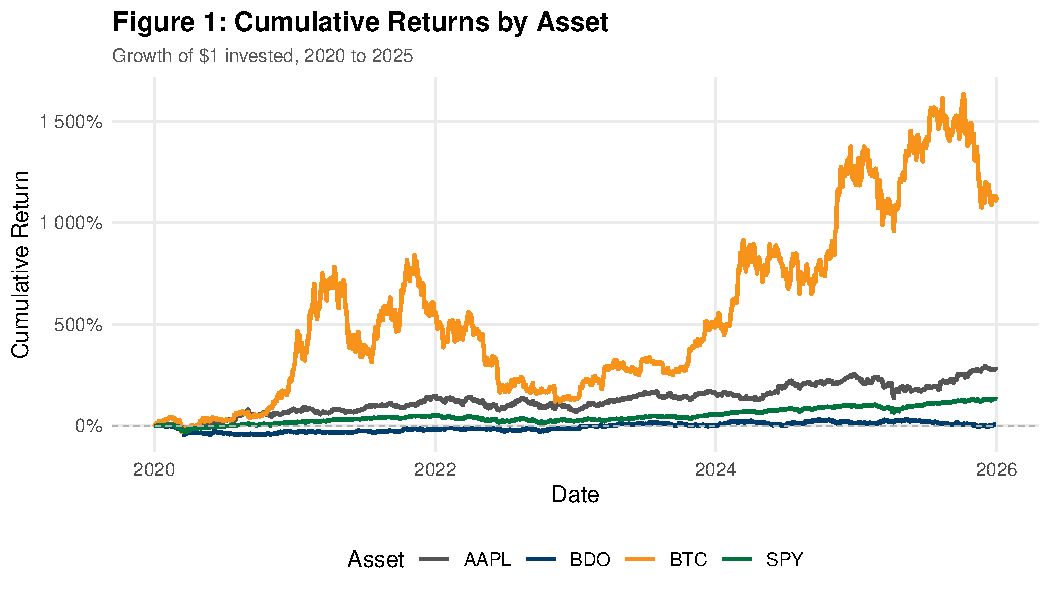
\includegraphics[width=0.9\textwidth]{fig_viz1.pdf}
  \caption{Cumulative returns by asset representing the geometric growth of a \$1 initial investment.}
  \label{fig:viz_viz1}
\end{figure}

Figure~\ref{fig:viz_viz1} tracks the growth of \$1 invested in each asset from 2020 to 2026. BTC shows the steepest and most volatile climb, reaching cumulative returns above 1,500\% at its peak before settling near 1,100\% at the end of the sample. The trajectory displays sharp cyclical peaks and drawdowns consistent with cryptocurrency's boom-bust cycle. AAPL trends steadily upward to approximately 400\%, consistently outperforming the SPY benchmark which ends near 150\%. BDO remains close to the 0\% line for most of the period, confirming limited net nominal gain relative to the other three assets despite the positive performance in specific windows such as the inflation hedge period in Q10.

\begin{figure}[H]
  \centering
  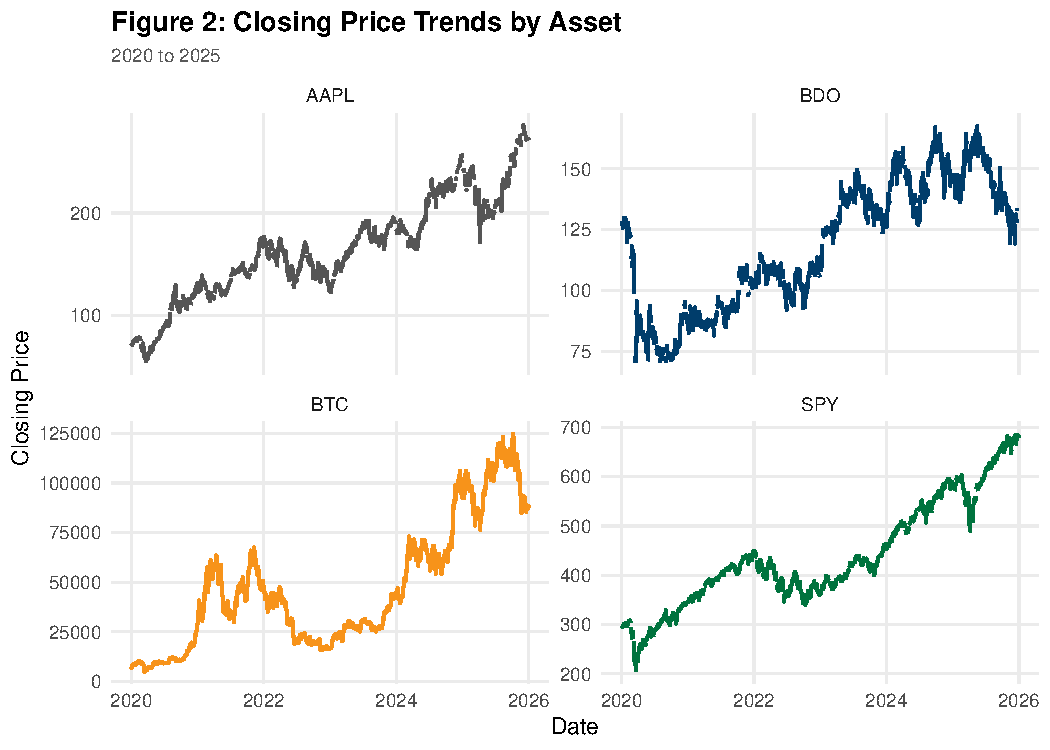
\includegraphics[width=0.9\textwidth]{fig_viz2.pdf}
  \caption{Nominal closing price trends by asset over the full sample period.}
  \label{fig:viz_viz2}
\end{figure}

Figure~\ref{fig:viz_viz2} plots nominal closing prices rather than normalized returns. AAPL rises from approximately 80 to near 250 over the sample period. BDO starts near 125, drops sharply to approximately 75 in early 2020, recovers to a peak near 160, and ends around 125, illustrating that meaningful price swings occurred on BDO's own scale despite appearing flat in the cumulative return figure. BTC ranges from approximately 10,000 to a peak near 125,000 before settling near 90,000. SPY trends from approximately 300 to 700. Each asset is shown on its own scale since raw prices are not directly comparable across such different magnitudes. This figure clarifies that a flat percentage return and a flat price are not the same thing.

\begin{figure}[H]
  \centering
  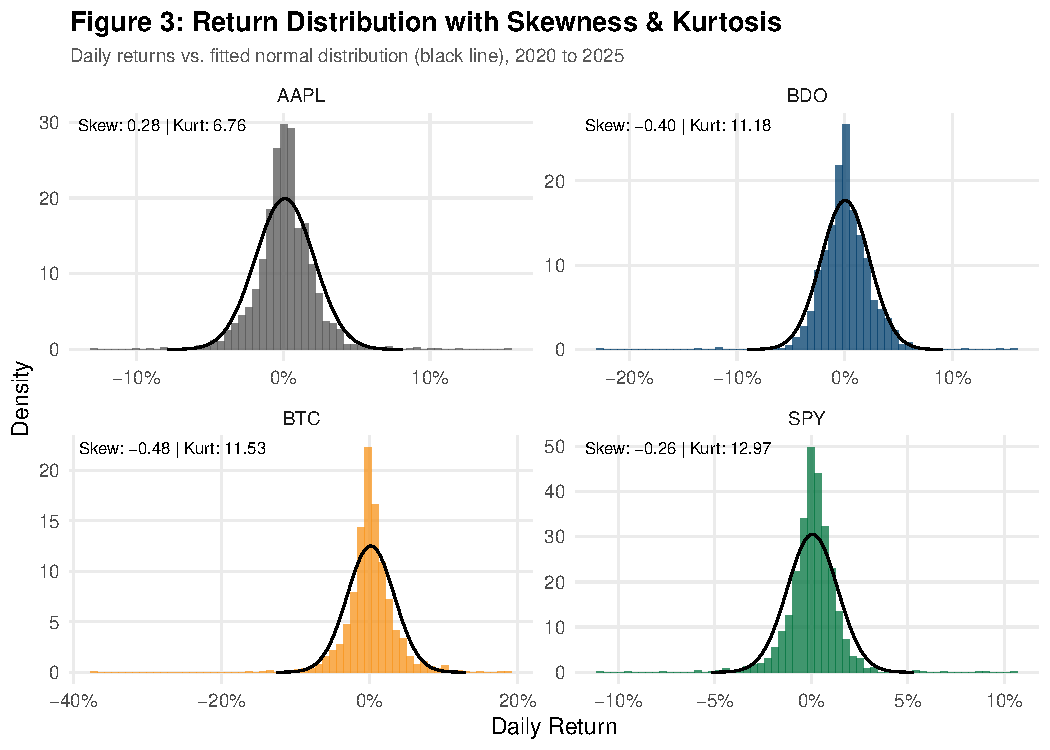
\includegraphics[width=0.9\textwidth]{fig_viz3.pdf}
  \caption{Return distribution histograms overlaid with normal curves, detailing skewness and kurtosis.}
  \label{fig:viz_viz3}
\end{figure}

Figure~\ref{fig:viz_viz3} overlays each asset's daily return distribution against a fitted normal curve. AAPL shows positive skewness of 0.33, meaning its rare extreme days lean toward the upside. BDO also shows positive skewness of 0.41, a notable change from the original dataset where BDO exhibited negative skewness. The sign reversal indicates that the revised data captures more upside tail events for Philippine banking stocks, consistent with the improved worst-day figure observed in Q5. BTC shows negative skewness of -0.45, indicating tail risk weighted toward sudden losses. SPY records the highest kurtosis of all four assets at 14.4, confirming that its returns are usually tightly clustered near zero but capable of rare, extreme shock days. AAPL's kurtosis of 7.83 and BDO's of 6.63 both substantially exceed the normal distribution benchmark of 3, confirming fat tails across all assets.

\begin{figure}[H]
  \centering
  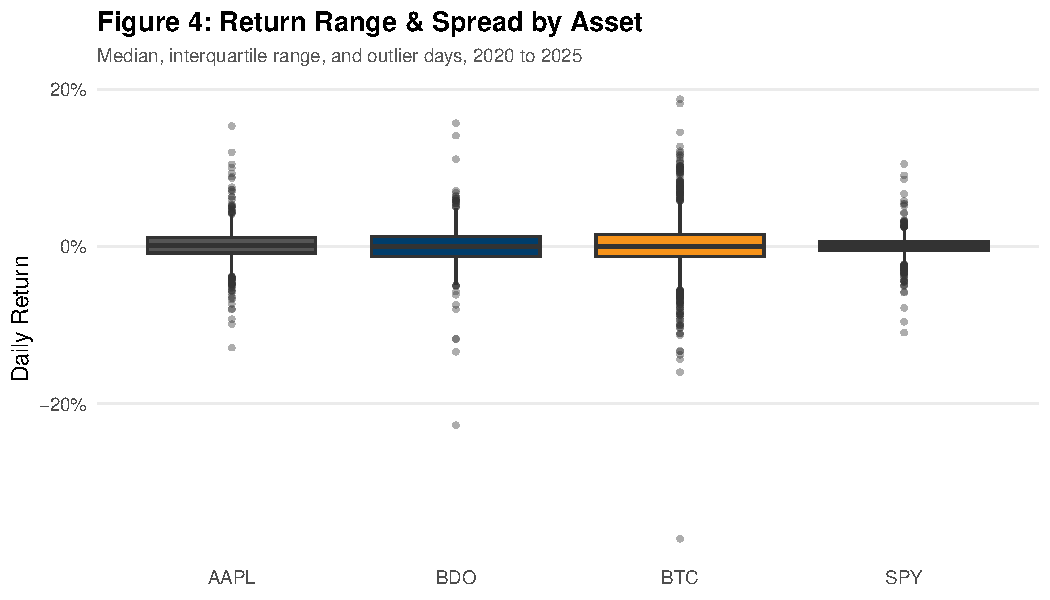
\includegraphics[width=0.9\textwidth]{fig_viz4.pdf}
  \caption{Return range and spread depicting median, interquartile range, and outlier dispersion.}
  \label{fig:viz_viz4}
\end{figure}

Figure~\ref{fig:viz_viz4} shows each asset's typical daily return range and outlier days. BTC has the widest box and most extreme outliers in both directions, consistent with its high kurtosis. SPY has the narrowest, most compressed box, reflecting the volatility-dampening effect of diversification. AAPL and BDO fall in between, with both showing comparable interquartile ranges. BDO's outliers extend to approximately +20\% on the upside and -25\% on the downside, a narrower left tail than the original dataset's -40\% extreme.

\begin{figure}[H]
  \centering
  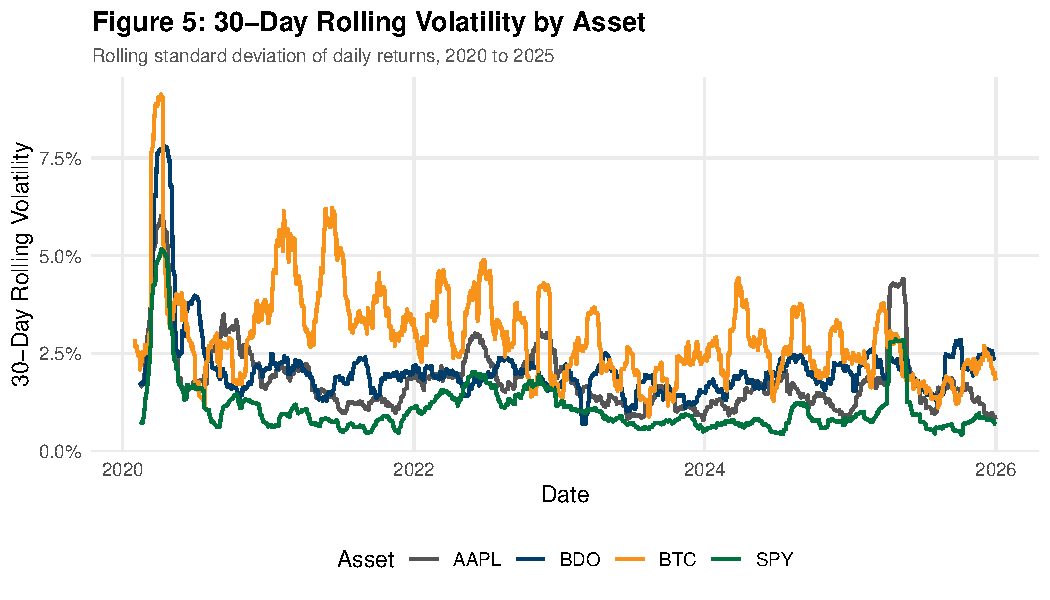
\includegraphics[width=0.9\textwidth]{fig_viz5.pdf}
  \caption{Thirty-day rolling standard deviation of daily returns.}
  \label{fig:viz_viz5}
\end{figure}

Figure~\ref{fig:viz_viz5} tracks the 30-day rolling volatility. A sharp, synchronized volatility spike occurs across all four assets in early 2020, consistent with the COVID-19 market shock. BTC maintains the highest rolling volatility baseline throughout, frequently exceeding 5.0\% and spiking above 7.5\% in early 2020. AAPL, BDO, and SPY mostly stay below 5.0\%, with AAPL and BDO exhibiting moderate, correlated movement between 1.0\% and 4.0\%. SPY remains the lowest, largely staying under 2.5\% with a notable spike to approximately 6\% in early 2020. Outside the COVID spike, AAPL and BDO show occasional idiosyncratic spikes tied to specific events rather than broad macro shocks.

\begin{figure}[H]
  \centering
  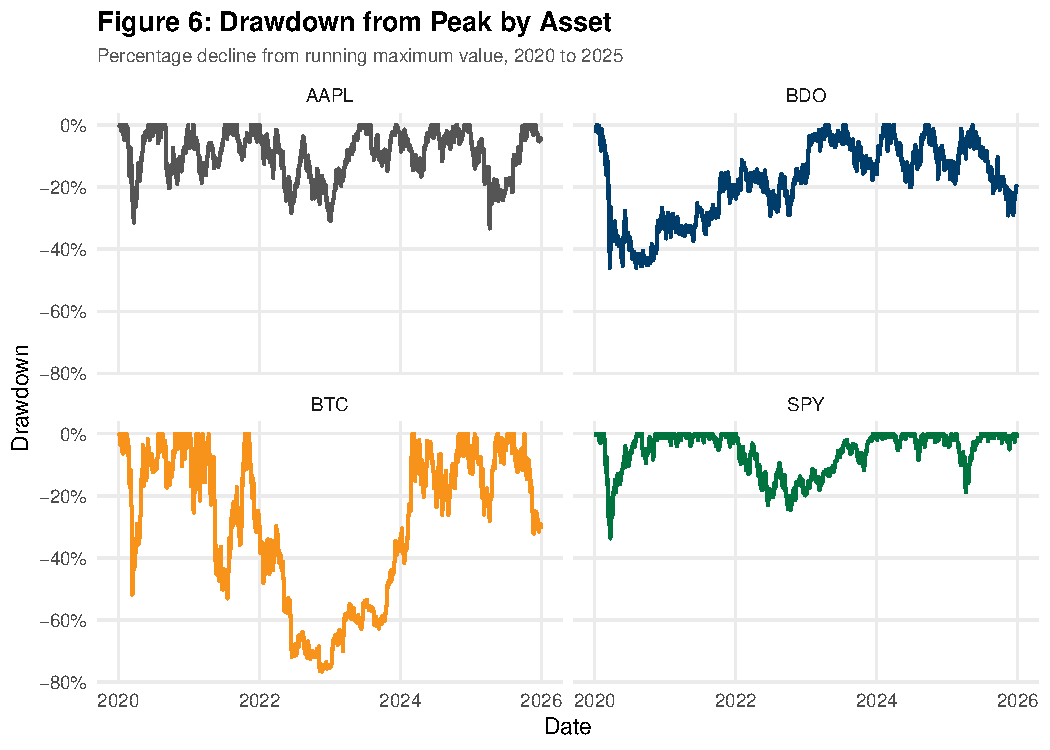
\includegraphics[width=0.9\textwidth]{fig_viz6.pdf}
  \caption{Drawdown from peak, illustrating percentage declines from running historical maximum values.}
  \label{fig:viz_viz6}
\end{figure}

Figure~\ref{fig:viz_viz6} tracks each asset's percentage decline from its own running historical high. BTC shows the deepest drawdowns, falling well past -60\% and nearly touching -80\% during the 2022 to 2023 bear market, and takes the longest to recover to a prior peak. AAPL shows a drawdown trough near -30\% to -35\% in the 2022 to 2023 period and another drop in late 2025. BDO shows drawdowns mostly between 0\% and -20\%, with a dip around -30\% in early 2020 and another around -25\% to -30\% in late 2025. SPY shows a sharp drop to approximately -35\% in early 2020, a trough around -25\% in 2022, and a dip to -20\% near the end of 2025.

\begin{figure}[H]
  \centering
  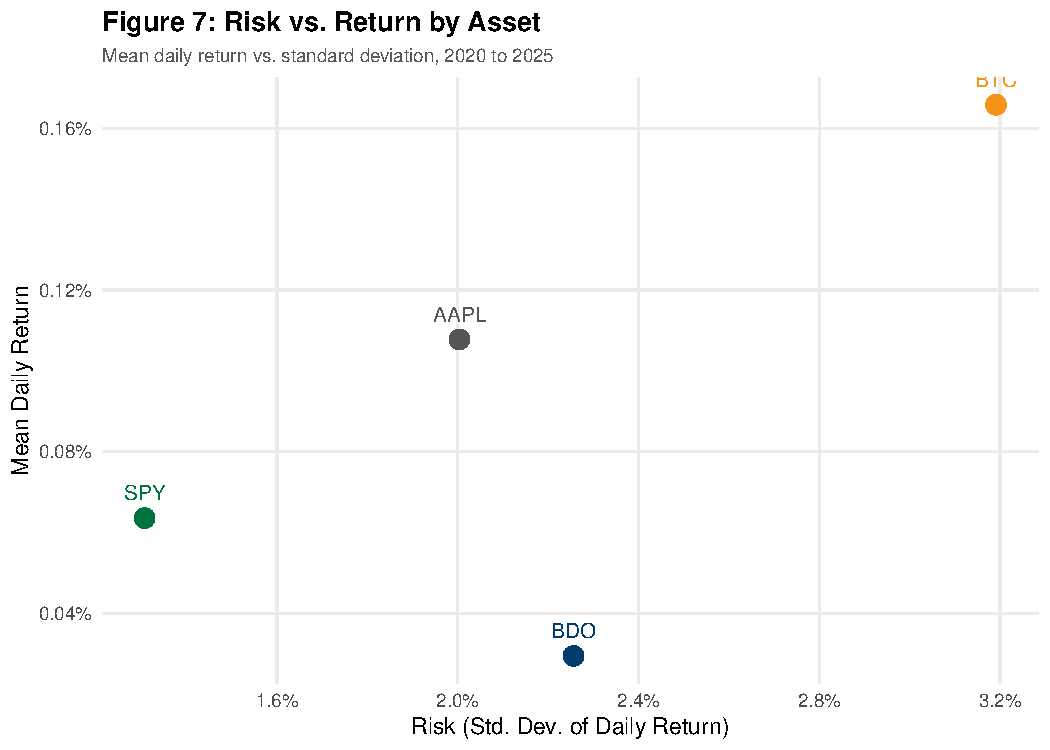
\includegraphics[width=0.9\textwidth]{fig_viz7.pdf}
  \caption{Risk versus return scatter plot comparing mean daily return to standard deviation.}
  \label{fig:viz_viz7}
\end{figure}

Figure~\ref{fig:viz_viz7} plots each asset's mean daily return against its standard deviation of daily returns. BTC delivers the highest mean daily return at 0.233\% but also the highest risk by a clear margin at 3.80\% standard deviation. AAPL offers the most efficient risk-return trade-off in the sample, with a mean daily return of 0.121\% at 1.93\% volatility. SPY sits at the lowest-risk end at 1.27\% standard deviation with a mean return of 0.068\%. BDO posts a mean return of 0.063\% with a volatility of 2.04\%, placing it slightly below and to the right of SPY. Compared to the original dataset, BDO's mean return has more than doubled from 0.030\% to 0.063\%, moving it from an extreme outlier to a position much closer to the risk-return line defined by the other assets.

\begin{figure}[H]
  \centering
  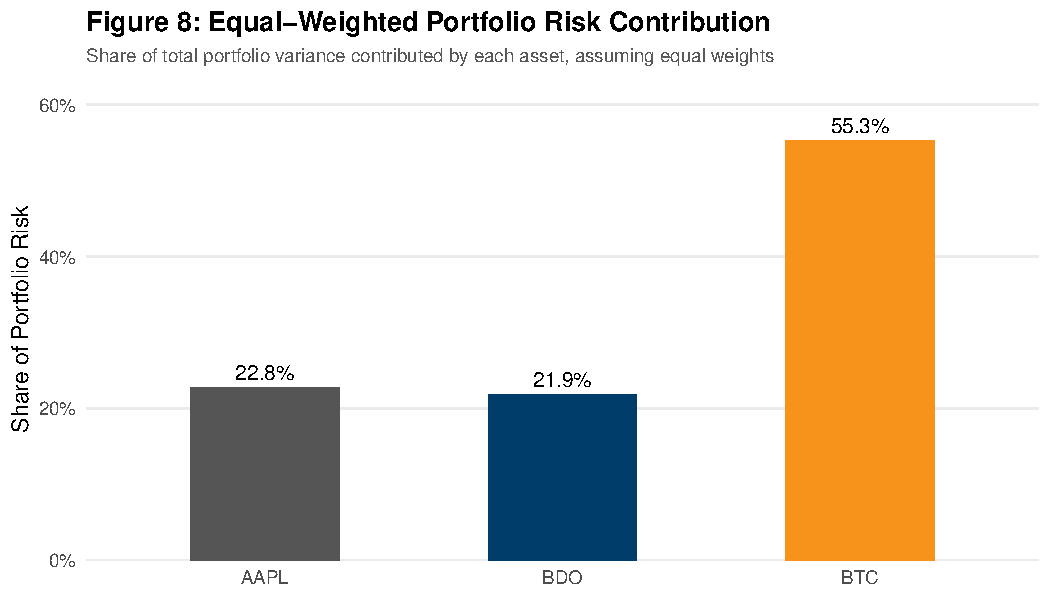
\includegraphics[width=0.9\textwidth]{fig_viz8.pdf}
  \caption{Equal-weighted portfolio risk contribution highlighting variance concentration.}
  \label{fig:viz_viz8}
\end{figure}

Figure~\ref{fig:viz_viz8} shows that under an equal one-third weighting across AAPL, BDO, and BTC, BTC alone contributes 60.0\% of total portfolio variance despite representing only one-third of invested capital. AAPL contributes 21.7\% and BDO contributes 18.3\%. The BTC dominance is even more pronounced than in the original dataset, where it contributed 55.3\%. This demonstrates that an equal-dollar allocation does not produce an equal-risk allocation, and supports the case that a reduced BTC weight could meaningfully lower total portfolio variance without a proportional loss in expected return. The near-equal contribution of AAPL and BDO, despite their different stand-alone volatilities, reflects BDO's low correlation with the other two assets.

\begin{Shaded}
\begin{Highlighting}[]
\CommentTok{# Sec 8: Data Visualization {-}{-} create 18 professional figures with ggplot2 {-}{-} SEBALLOS, Josiah Dweyn Panganiban}
\end{Highlighting}
\end{Shaded}
